The model is trained with PyTorch 1.10.2, CUDA 10.2.89, GPU with single NVIDIA GEFORCE GTX 1080Ti.


%% nnn24 exp
\section{Neighbor Input}


%% nnnn exp
\section{Normal Neural Network}
The first neural network that worked well for normal prediction in this master thesis is introduced in this section. It is simply named Normal Neural Network, or NNN. The input is 512x512x3 3D vertex matrix and output is 512x512x3 normal map. The architecture is based on UNet \cite{unet} with 3 times downsampling and 3 times upsampling. Gated convolution layer is used as a substitution for standard convolution layer in order to handle the sparse input. The channel size is 32 through the whole network unless the last one.  
For the training detail, this model is trained on the whole dataset with 500 items, with learning rate 0.001, penalty 1.4. The model architecture is shown in Figure \ref{fig:nnnn_archi}


\begin{figure}[!h]
	\centering
	
	%% https://tex.stackexchange.com/questions/12020/what-is-the-easiest-way-to-draw-a-3d-cube-with-tikz
	\begin{tikzpicture}
		%% -------------------------------------- parameters ------------------------------------------------
		\pgfmathsetmacro{\vdist}{0.4}
		
		\pgfmathsetmacro{\boxsizea}{3}	%% width 512
		\pgfmathsetmacro{\boxsizeb}{1.5}	%% width 256
		\pgfmathsetmacro{\boxsizec}{1}	%% width 128
		\pgfmathsetmacro{\boxsized}{0.7}	%% width 64
		
		
		\pgfmathsetmacro{\boxwidthd}{0.1}	%% width 1
		\pgfmathsetmacro{\boxwidtha}{0.2}	%% width 3
		\pgfmathsetmacro{\boxwidthb}{\boxwidtha*1.3}	%% width 32
		\pgfmathsetmacro{\boxwidthc}{\boxwidtha*3}		%% width 64
		
		\pgfmathsetmacro{\convwshift}{9}
		\pgfmathsetmacro{\preprocessingshift}{4}
		\pgfmathsetmacro{\labelshift}{1.5}
		\pgfmathsetmacro{\gconvwshift}{0}
		
		\pgfmathsetmacro{\secrowshift}{-6}
		
		\pgfmathsetmacro{\convrowstart}{4}
		\pgfmathsetmacro{\secondrowstart}{4}

		%% https://www.tug.org/pracjourn/2007-4/walden/color.pdf
		\definecolor{gconvcolor}{rgb}{0.5,0.7,0.7}
		\definecolor{convcolor}{rgb}{0.5,0.7,0.3}
		\definecolor{gconvdilatedcolor}{rgb}{0.6,0,0.3}
		
		
		%% ---------------------------------- preprocessing --------------------------------------------
		%%  img_in 1x512x512
		\pgfmathsetmacro{\disttimes}{3.5}
		\pgfmathsetmacro{\yschift}{\preprocessingshift}
		\node[inner sep=0pt] (depthmap) at (\vdist*\disttimes,\yschift)
		{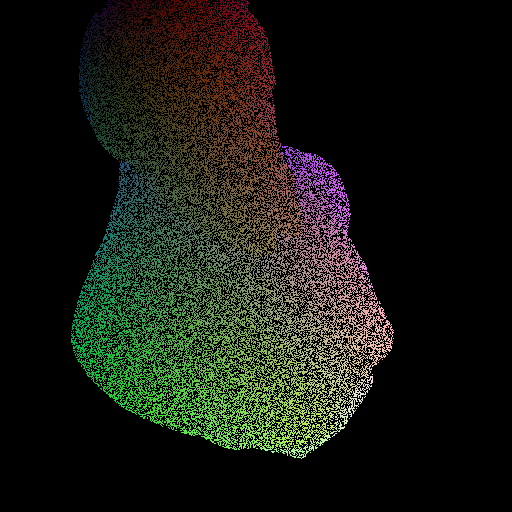
\includegraphics[width=.15\textwidth]{./pic/00440.vertex.png}};
		\node[text width=3.5cm] at (\vdist*\disttimes+1,\yschift-1.5) {3D Vertex};
		
		\draw [-stealth](1.45,\yschift-1.8) -- (1.45,\yschift-2.6);
		
		\draw [-stealth]  (\vdist*\disttimes+1.6,\yschift) -- (\vdist*\disttimes+1.1,\yschift);
		
		\pgfmathsetmacro{\disttimes}{10}
		\pgfmathsetmacro{\yschift}{\preprocessingshift}
		\node[inner sep=0pt] (depthmap) at (\vdist*\disttimes,\yschift)
		{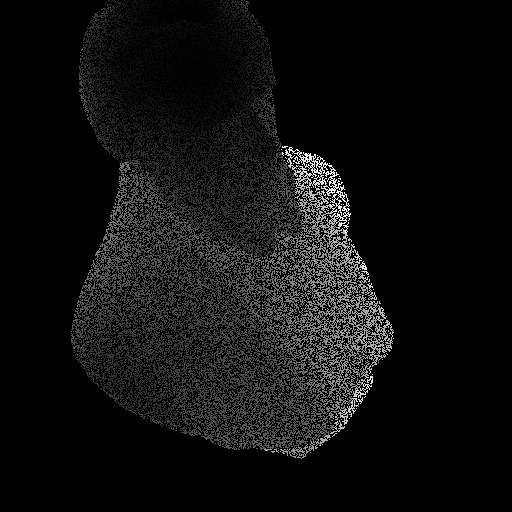
\includegraphics[width=.15\textwidth]{./pic/00440.depth0_noise.png}};
		\node[text width=3.5cm] at (\vdist*\disttimes+1,\yschift-1.5) {Add Noise};
		
		\draw [-stealth] (\vdist*\disttimes+1.6,\yschift) -- (\vdist*\disttimes+1.1,\yschift);
		
		\pgfmathsetmacro{\disttimes}{16.5}
		\pgfmathsetmacro{\yschift}{\preprocessingshift}
		\node[inner sep=0pt] (depthmap) at (\vdist*\disttimes,\yschift)
		{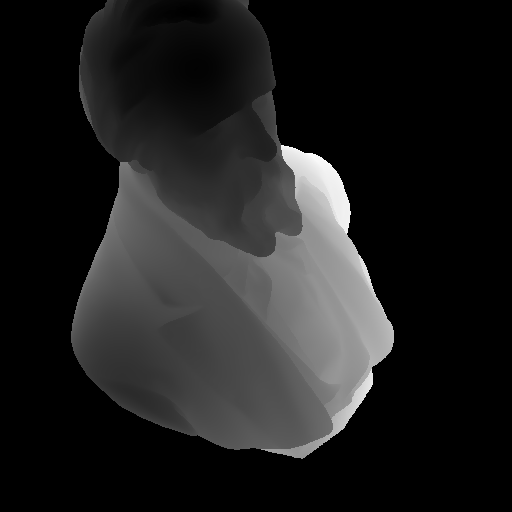
\includegraphics[width=.15\textwidth]{./pic/00440.depth0.png}};
		\node[text width=2cm] at (\vdist*\disttimes+0.2,\yschift-1.5) {Depth Map};
		
		
		%% ----------------------------------- output normal map -------------------------------------
		\pgfmathsetmacro{\disttimes}{31}
		\pgfmathsetmacro{\yschift}{\preprocessingshift}
		\node[inner sep=0pt] (depthmap) at (\vdist*\disttimes,\yschift)
		{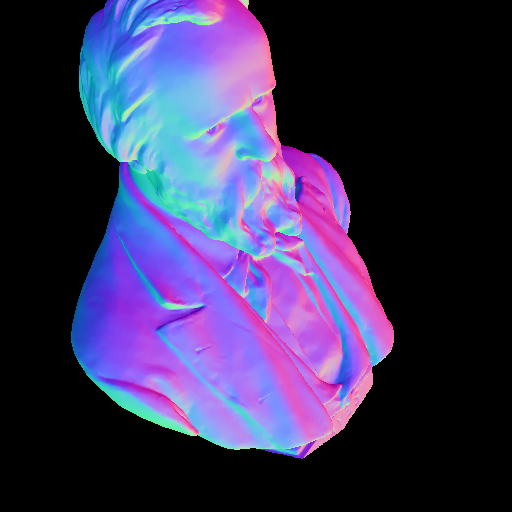
\includegraphics[width=.15\textwidth]{./pic/00440.normal0.png}};
		\node[text width=2cm] at (\vdist*\disttimes,\yschift-1.5) {Normal Map};
		
		\draw [-stealth] (\vdist*\disttimes+0.2,\yschift-2.7) -- (\vdist*\disttimes+0.2,\yschift-1.8);
		
		
		%% ------------------------------------------- vertex input ----------------------------------------------
		%% 	d_in							3x512x512
		%%	dconv1: 	d_in-->x1 			32x512x512
		\pgfmathsetmacro{\disttimes}{1}	%% width 32
		\pgfmathsetmacro{\boxsize}{\boxsizea}	%% size 512
		\pgfmathsetmacro{\boxwidth}{\boxwidthb}	%% width 32
		\pgfmathsetmacro{\yschift}{\gconvwshift}
		\node[text width=1cm] at (\vdist*\disttimes+0.1,\yschift-3.5) {32};
		\draw[black, fill=gconvcolor] (\vdist*\disttimes,\yschift,0) -- ++(-\boxwidth,0,0) -- ++(0,-\boxsize,0) -- ++(\boxwidth,0,0) -- cycle;
		\draw[black, fill=gconvcolor] (\vdist*\disttimes,\yschift,0) -- ++(0,0,-\boxsize) -- ++(0,-\boxsize,0) -- ++(0,0,\boxsize) -- cycle;
		\draw[black, fill=gconvcolor] (\vdist*\disttimes,\yschift,0) -- ++(-\boxwidth,0,0) -- ++(0,0,-\boxsize) -- ++(\boxwidth,0,0) -- cycle;
		
		%%	dconv2:		x1-->x1				32x512x512
		\pgfmathsetmacro{\disttimes}{2}	%% width 32
		\pgfmathsetmacro{\boxsize}{\boxsizea}	%% size 512
		\pgfmathsetmacro{\boxwidth}{\boxwidthb}	%% width 32
		\pgfmathsetmacro{\yschift}{\gconvwshift}
		\draw[black, fill=gconvcolor] (\vdist*\disttimes,\yschift,0) -- ++(-\boxwidth,0,0) -- ++(0,-\boxsize,0) -- ++(\boxwidth,0,0) -- cycle;
		\draw[black, fill=gconvcolor] (\vdist*\disttimes,\yschift,0) -- ++(0,0,-\boxsize) -- ++(0,-\boxsize,0) -- ++(0,0,\boxsize) -- cycle;
		\draw[black, fill=gconvcolor] (\vdist*\disttimes,\yschift,0) -- ++(-\boxwidth,0,0) -- ++(0,0,-\boxsize) -- ++(\boxwidth,0,0) -- cycle;
		
		%%	dconv3:		x1-->x1				32x512x512
		\pgfmathsetmacro{\disttimes}{3}	%% width 32
		\pgfmathsetmacro{\boxsize}{\boxsizea}	%% size 512
		\pgfmathsetmacro{\boxwidth}{\boxwidthb}	%% width 32
		\pgfmathsetmacro{\yschift}{\gconvwshift}
		\draw[black, fill=gconvcolor] (\vdist*\disttimes,\yschift,0) -- ++(-\boxwidth,0,0) -- ++(0,-\boxsize,0) -- ++(\boxwidth,0,0) -- cycle;
		\draw[black, fill=gconvcolor] (\vdist*\disttimes,\yschift,0) -- ++(0,0,-\boxsize) -- ++(0,-\boxsize,0) -- ++(0,0,\boxsize) -- cycle;
		\draw[black, fill=gconvcolor] (\vdist*\disttimes,\yschift,0) -- ++(-\boxwidth,0,0) -- ++(0,0,-\boxsize) -- ++(\boxwidth,0,0) -- cycle;
		
		\draw (\vdist*\disttimes-0.2,\yschift-3.2) -- (\vdist*\disttimes-0.2,\yschift-4);
		\draw (\vdist*\disttimes-0.2,\yschift-4) -- (\vdist*\disttimes+9,\yschift-4);
		\draw [-stealth] (\vdist*\disttimes+9,\yschift-4) -- (\vdist*\disttimes+9,\yschift-3.2);
		
		
		%% downsample 1
		%%	dconv4:		x1-->x2				32x256x256
		\pgfmathsetmacro{\disttimes}{4}	%% width 32
		\pgfmathsetmacro{\boxsize}{\boxsizeb}	%% size 256
		\pgfmathsetmacro{\boxwidth}{\boxwidthb}	%% width 32
		\pgfmathsetmacro{\yschift}{\gconvwshift-0.5}	%% width 32
		\draw[black, fill=gconvcolor] (\vdist*\disttimes,\yschift,0) -- ++(-\boxwidth,0,0) -- ++(0,-\boxsize,0) -- ++(\boxwidth,0,0) -- cycle;
		\draw[black, fill=gconvcolor] (\vdist*\disttimes,\yschift,0) -- ++(0,0,-\boxsize) -- ++(0,-\boxsize,0) -- ++(0,0,\boxsize) -- cycle;
		\draw[black, fill=gconvcolor] (\vdist*\disttimes,\yschift,0) -- ++(-\boxwidth,0,0) -- ++(0,0,-\boxsize) -- ++(\boxwidth,0,0) -- cycle;
		%%	dconv2:		x2-->x2				32x256x256
		\pgfmathsetmacro{\disttimes}{5}	%% width 32
		\pgfmathsetmacro{\boxsize}{\boxsizeb}	%% size 256
		\pgfmathsetmacro{\boxwidth}{\boxwidthb}	%% width 32
		\pgfmathsetmacro{\yschift}{\gconvwshift-0.5}	%% width 32
		\draw[black, fill=gconvcolor] (\vdist*\disttimes,\yschift,0) -- ++(-\boxwidth,0,0) -- ++(0,-\boxsize,0) -- ++(\boxwidth,0,0) -- cycle;
		\draw[black, fill=gconvcolor] (\vdist*\disttimes,\yschift,0) -- ++(0,0,-\boxsize) -- ++(0,-\boxsize,0) -- ++(0,0,\boxsize) -- cycle;
		\draw[black, fill=gconvcolor] (\vdist*\disttimes,\yschift,0) -- ++(-\boxwidth,0,0) -- ++(0,0,-\boxsize) -- ++(\boxwidth,0,0) -- cycle;
		%%	dconv3:		x2-->x2				32x256x256
		\pgfmathsetmacro{\disttimes}{6}	%% width 32
		\pgfmathsetmacro{\boxsize}{\boxsizeb}	%% size 256
		\pgfmathsetmacro{\boxwidth}{\boxwidthb}	%% width 32
		\pgfmathsetmacro{\yschift}{\gconvwshift-0.5}	%% width 32
		\draw[black, fill=gconvcolor] (\vdist*\disttimes,\yschift,0) -- ++(-\boxwidth,0,0) -- ++(0,-\boxsize,0) -- ++(\boxwidth,0,0) -- cycle;
		\draw[black, fill=gconvcolor] (\vdist*\disttimes,\yschift,0) -- ++(0,0,-\boxsize) -- ++(0,-\boxsize,0) -- ++(0,0,\boxsize) -- cycle;
		\draw[black, fill=gconvcolor] (\vdist*\disttimes,\yschift,0) -- ++(-\boxwidth,0,0) -- ++(0,0,-\boxsize) -- ++(\boxwidth,0,0) -- cycle;
		
		\draw (\vdist*\disttimes-0.1,\yschift-1.6) -- (\vdist*\disttimes-0.1,\yschift-2.7);
		\draw (\vdist*\disttimes-0.1,\yschift-2.7) -- (\vdist*\disttimes+6.5,\yschift-2.7);
		\draw [-stealth] (\vdist*\disttimes+6.5,\yschift-2.7) -- (\vdist*\disttimes+6.5,\yschift-1.7);
		
		
		%% downsample 2
		%%	dconv4:		x2-->x3				32x128x128
		\pgfmathsetmacro{\disttimes}{7}	%% width 32
		\pgfmathsetmacro{\boxsize}{\boxsizec}	%% size 128
		\pgfmathsetmacro{\boxwidth}{\boxwidthb}	%% width 32
		\pgfmathsetmacro{\yschift}{\gconvwshift-0.8}	%% width 32
		\draw[black, fill=gconvcolor] (\vdist*\disttimes,\yschift,0) -- ++(-\boxwidth,0,0) -- ++(0,-\boxsize,0) -- ++(\boxwidth,0,0) -- cycle;
		\draw[black, fill=gconvcolor] (\vdist*\disttimes,\yschift,0) -- ++(0,0,-\boxsize) -- ++(0,-\boxsize,0) -- ++(0,0,\boxsize) -- cycle;
		\draw[black, fill=gconvcolor] (\vdist*\disttimes,\yschift,0) -- ++(-\boxwidth,0,0) -- ++(0,0,-\boxsize) -- ++(\boxwidth,0,0) -- cycle;
		%%	dconv2:		x3-->x3				32x128x128
		\pgfmathsetmacro{\disttimes}{8}	%% width 32
		\pgfmathsetmacro{\boxsize}{\boxsizec}	%% size 128
		\pgfmathsetmacro{\boxwidth}{\boxwidthb}	%% width 32
		\pgfmathsetmacro{\yschift}{\gconvwshift-0.8}	%% width 32
		\draw[black, fill=gconvcolor] (\vdist*\disttimes,\yschift,0) -- ++(-\boxwidth,0,0) -- ++(0,-\boxsize,0) -- ++(\boxwidth,0,0) -- cycle;
		\draw[black, fill=gconvcolor] (\vdist*\disttimes,\yschift,0) -- ++(0,0,-\boxsize) -- ++(0,-\boxsize,0) -- ++(0,0,\boxsize) -- cycle;
		\draw[black, fill=gconvcolor] (\vdist*\disttimes,\yschift,0) -- ++(-\boxwidth,0,0) -- ++(0,0,-\boxsize) -- ++(\boxwidth,0,0) -- cycle;
		%%	dconv3:		x3-->x3				32x128x128
		\pgfmathsetmacro{\disttimes}{9}	%% width 32
		\pgfmathsetmacro{\boxsize}{\boxsizec}	%% size 128
		\pgfmathsetmacro{\boxwidth}{\boxwidthb}	%% width 32
		\pgfmathsetmacro{\yschift}{\gconvwshift-0.8}	%% width 32
		\draw[black, fill=gconvcolor] (\vdist*\disttimes,\yschift,0) -- ++(-\boxwidth,0,0) -- ++(0,-\boxsize,0) -- ++(\boxwidth,0,0) -- cycle;
		\draw[black, fill=gconvcolor] (\vdist*\disttimes,\yschift,0) -- ++(0,0,-\boxsize) -- ++(0,-\boxsize,0) -- ++(0,0,\boxsize) -- cycle;
		\draw[black, fill=gconvcolor] (\vdist*\disttimes,\yschift,0) -- ++(-\boxwidth,0,0) -- ++(0,0,-\boxsize) -- ++(\boxwidth,0,0) -- cycle;
		
		\draw (\vdist*\disttimes-0.1,\yschift-1.2) -- (\vdist*\disttimes-0.1,\yschift-1.8);
		\draw (\vdist*\disttimes-0.1,\yschift-1.8) -- (\vdist*\disttimes+4.2,\yschift-1.8);
		\draw [-stealth] (\vdist*\disttimes+4.2,\yschift-1.8) -- (\vdist*\disttimes+4.2,\yschift-1.2);
		
		
		%% downsample 3
		%%	dconv4:		x3-->x4				32x64x64
		\pgfmathsetmacro{\disttimes}{10}
		\pgfmathsetmacro{\boxsize}{\boxsized}	%% size 64
		\pgfmathsetmacro{\boxwidth}{\boxwidthb}	%% width 32
		\pgfmathsetmacro{\yschift}{\gconvwshift-1}
		\draw[black, fill=gconvcolor] (\vdist*\disttimes,\yschift,0) -- ++(-\boxwidth,0,0) -- ++(0,-\boxsize,0) -- ++(\boxwidth,0,0) -- cycle;
		\draw[black, fill=gconvcolor] (\vdist*\disttimes,\yschift,0) -- ++(0,0,-\boxsize) -- ++(0,-\boxsize,0) -- ++(0,0,\boxsize) -- cycle;
		\draw[black, fill=gconvcolor] (\vdist*\disttimes,\yschift,0) -- ++(-\boxwidth,0,0) -- ++(0,0,-\boxsize) -- ++(\boxwidth,0,0) -- cycle;
		%%	dconv2:		x4-->x4				32x64x64
		\pgfmathsetmacro{\disttimes}{11}
		\pgfmathsetmacro{\boxsize}{\boxsized}	%% size 64
		\pgfmathsetmacro{\boxwidth}{\boxwidthb}	%% width 32
		\pgfmathsetmacro{\yschift}{\gconvwshift-1}	%% width 32
		\draw[black, fill=gconvcolor] (\vdist*\disttimes,\yschift,0) -- ++(-\boxwidth,0,0) -- ++(0,-\boxsize,0) -- ++(\boxwidth,0,0) -- cycle;
		\draw[black, fill=gconvcolor] (\vdist*\disttimes,\yschift,0) -- ++(0,0,-\boxsize) -- ++(0,-\boxsize,0) -- ++(0,0,\boxsize) -- cycle;
		\draw[black, fill=gconvcolor] (\vdist*\disttimes,\yschift,0) -- ++(-\boxwidth,0,0) -- ++(0,0,-\boxsize) -- ++(\boxwidth,0,0) -- cycle;
		%%	dconv3:		x4-->x4				32x64x64
		\pgfmathsetmacro{\disttimes}{12}
		\pgfmathsetmacro{\boxsize}{\boxsized}	%% size 64
		\pgfmathsetmacro{\boxwidth}{\boxwidthb}	%% width 32
		\pgfmathsetmacro{\yschift}{\gconvwshift-1}	%% width 32
		\draw[black, fill=gconvcolor] (\vdist*\disttimes,\yschift,0) -- ++(-\boxwidth,0,0) -- ++(0,-\boxsize,0) -- ++(\boxwidth,0,0) -- cycle;
		\draw[black, fill=gconvcolor] (\vdist*\disttimes,\yschift,0) -- ++(0,0,-\boxsize) -- ++(0,-\boxsize,0) -- ++(0,0,\boxsize) -- cycle;
		\draw[black, fill=gconvcolor] (\vdist*\disttimes,\yschift,0) -- ++(-\boxwidth,0,0) -- ++(0,0,-\boxsize) -- ++(\boxwidth,0,0) -- cycle;
		
		%% dilated
		%%	dilated1:	x4-->x4				32x64x64
		\pgfmathsetmacro{\disttimes}{13}
		\pgfmathsetmacro{\boxsize}{\boxsized}	%% size 64
		\pgfmathsetmacro{\boxwidth}{\boxwidthb}	%% width 32
		\pgfmathsetmacro{\yschift}{\gconvwshift-1}	%% width 32
		\draw[black, fill=gconvdilatedcolor] (\vdist*\disttimes,\yschift,0) -- ++(-\boxwidth,0,0) -- ++(0,-\boxsize,0) -- ++(\boxwidth,0,0) -- cycle;
		\draw[black, fill=gconvdilatedcolor] (\vdist*\disttimes,\yschift,0) -- ++(0,0,-\boxsize) -- ++(0,-\boxsize,0) -- ++(0,0,\boxsize) -- cycle;
		\draw[black, fill=gconvdilatedcolor] (\vdist*\disttimes,\yschift,0) -- ++(-\boxwidth,0,0) -- ++(0,0,-\boxsize) -- ++(\boxwidth,0,0) -- cycle;
		%%	dilated2:	x4-->x4				32x64x64
		\pgfmathsetmacro{\disttimes}{14}
		\pgfmathsetmacro{\boxsize}{\boxsized}	%% size 64
		\pgfmathsetmacro{\boxwidth}{\boxwidthb}	%% width 32
		\pgfmathsetmacro{\yschift}{\gconvwshift-1}	%% width 32
		\draw[black, fill=gconvdilatedcolor] (\vdist*\disttimes,\yschift,0) -- ++(-\boxwidth,0,0) -- ++(0,-\boxsize,0) -- ++(\boxwidth,0,0) -- cycle;
		\draw[black, fill=gconvdilatedcolor] (\vdist*\disttimes,\yschift,0) -- ++(0,0,-\boxsize) -- ++(0,-\boxsize,0) -- ++(0,0,\boxsize) -- cycle;
		\draw[black, fill=gconvdilatedcolor] (\vdist*\disttimes,\yschift,0) -- ++(-\boxwidth,0,0) -- ++(0,0,-\boxsize) -- ++(\boxwidth,0,0) -- cycle;
		%%	dilated3:	x4-->x4				32x64x64
		\pgfmathsetmacro{\disttimes}{15}
		\pgfmathsetmacro{\boxsize}{\boxsized}	%% size 64
		\pgfmathsetmacro{\boxwidth}{\boxwidthb}	%% width 32
		\pgfmathsetmacro{\yschift}{\gconvwshift-1}	%% width 32
		\draw[black, fill=gconvdilatedcolor] (\vdist*\disttimes,\yschift,0) -- ++(-\boxwidth,0,0) -- ++(0,-\boxsize,0) -- ++(\boxwidth,0,0) -- cycle;
		\draw[black, fill=gconvdilatedcolor] (\vdist*\disttimes,\yschift,0) -- ++(0,0,-\boxsize) -- ++(0,-\boxsize,0) -- ++(0,0,\boxsize) -- cycle;
		\draw[black, fill=gconvdilatedcolor] (\vdist*\disttimes,\yschift,0) -- ++(-\boxwidth,0,0) -- ++(0,0,-\boxsize) -- ++(\boxwidth,0,0) -- cycle;
		%%	dilated4:	x4-->x4				32x64x64
		\pgfmathsetmacro{\disttimes}{16}
		\pgfmathsetmacro{\boxsize}{\boxsized}	%% size 64
		\pgfmathsetmacro{\boxwidth}{\boxwidthb}	%% width 32
		\pgfmathsetmacro{\yschift}{\gconvwshift-1}	%% width 32
		\draw[black, fill=gconvdilatedcolor] (\vdist*\disttimes,\yschift,0) -- ++(-\boxwidth,0,0) -- ++(0,-\boxsize,0) -- ++(\boxwidth,0,0) -- cycle;
		\draw[black, fill=gconvdilatedcolor] (\vdist*\disttimes,\yschift,0) -- ++(0,0,-\boxsize) -- ++(0,-\boxsize,0) -- ++(0,0,\boxsize) -- cycle;
		\draw[black, fill=gconvdilatedcolor] (\vdist*\disttimes,\yschift,0) -- ++(-\boxwidth,0,0) -- ++(0,0,-\boxsize) -- ++(\boxwidth,0,0) -- cycle;
		%%	dconv2:		x4-->x4				32x64x64
		\pgfmathsetmacro{\disttimes}{17}
		\pgfmathsetmacro{\boxsize}{\boxsized}	%% size 64
		\pgfmathsetmacro{\boxwidth}{\boxwidthb}	%% width 32
		\pgfmathsetmacro{\yschift}{\gconvwshift-1}	%% width 32
		\draw[black, fill=gconvcolor] (\vdist*\disttimes,\yschift,0) -- ++(-\boxwidth,0,0) -- ++(0,-\boxsize,0) -- ++(\boxwidth,0,0) -- cycle;
		\draw[black, fill=gconvcolor] (\vdist*\disttimes,\yschift,0) -- ++(0,0,-\boxsize) -- ++(0,-\boxsize,0) -- ++(0,0,\boxsize) -- cycle;
		\draw[black, fill=gconvcolor] (\vdist*\disttimes,\yschift,0) -- ++(-\boxwidth,0,0) -- ++(0,0,-\boxsize) -- ++(\boxwidth,0,0) -- cycle;
		%%	dconv3:		x4-->x4				32x64x64
		\pgfmathsetmacro{\disttimes}{18}
		\pgfmathsetmacro{\boxsize}{\boxsized}	%% size 64
		\pgfmathsetmacro{\boxwidth}{\boxwidthb}	%% width 32
		\pgfmathsetmacro{\yschift}{\gconvwshift-1}	%% width 32
		\draw[black, fill=gconvcolor] (\vdist*\disttimes,\yschift,0) -- ++(-\boxwidth,0,0) -- ++(0,-\boxsize,0) -- ++(\boxwidth,0,0) -- cycle;
		\draw[black, fill=gconvcolor] (\vdist*\disttimes,\yschift,0) -- ++(0,0,-\boxsize) -- ++(0,-\boxsize,0) -- ++(0,0,\boxsize) -- cycle;
		\draw[black, fill=gconvcolor] (\vdist*\disttimes,\yschift,0) -- ++(-\boxwidth,0,0) -- ++(0,0,-\boxsize) -- ++(\boxwidth,0,0) -- cycle;

		
		%% ----------------------------------- upsampling -------------------------------------
		
		%% upsample 1
		%% interpolate	x4-->x3_us			64x128x128
		\pgfmathsetmacro{\disttimes}{19}
		\pgfmathsetmacro{\boxsize}{\boxsizec}	%% size 128
		\pgfmathsetmacro{\boxwidth}{\boxwidthb}	%% width 32
		\pgfmathsetmacro{\yschift}{\gconvwshift-0.9}	%% width 32
		\draw[black, fill=gconvcolor] (\vdist*\disttimes,\yschift,0) -- ++(-\boxwidth,0,0) -- ++(0,-\boxsize,0) -- ++(\boxwidth,0,0) -- cycle;
		\draw[black, fill=gconvcolor] (\vdist*\disttimes,\yschift,0) -- ++(0,0,-\boxsize) -- ++(0,-\boxsize,0) -- ++(0,0,\boxsize) -- cycle;
		\draw[black, fill=gconvcolor] (\vdist*\disttimes,\yschift,0) -- ++(-\boxwidth,0,0) -- ++(0,0,-\boxsize) -- ++(\boxwidth,0,0) -- cycle;

		%% concatenate x3_us
		\pgfmathsetmacro{\boxsize}{\boxsizec}	%% size 128
		\pgfmathsetmacro{\boxwidth}{\boxwidthb}	%% width 32
		\pgfmathsetmacro{\yschift}{\gconvwshift-0.9}	%% width 32
		\draw[black, fill=gconvcolor] (\vdist*\disttimes+\boxwidth,\yschift,0) -- ++(-\boxwidth,0,0) -- ++(0,-\boxsize,0) -- ++(\boxwidth,0,0) -- cycle;
		\draw[black, fill=gconvcolor] (\vdist*\disttimes+\boxwidth,\yschift,0) -- ++(0,0,-\boxsize) -- ++(0,-\boxsize,0) -- ++(0,0,\boxsize) -- cycle;
		\draw[black, fill=gconvcolor] (\vdist*\disttimes+\boxwidth,\yschift,0) -- ++(-\boxwidth,0,0) -- ++(0,0,-\boxsize) -- ++(\boxwidth,0,0) -- cycle;
		
		%% uconv1		x3_us-->x3			32x128x128
		\pgfmathsetmacro{\disttimes}{21}
		\pgfmathsetmacro{\boxsize}{\boxsizec}	%% size 128
		\pgfmathsetmacro{\boxwidth}{\boxwidthb}	%% width 32
		\pgfmathsetmacro{\yschift}{\gconvwshift-0.9}	%% width 32
		\draw[black, fill=gconvcolor] (\vdist*\disttimes,\yschift,0) -- ++(-\boxwidth,0,0) -- ++(0,-\boxsize,0) -- ++(\boxwidth,0,0) -- cycle;
		\draw[black, fill=gconvcolor] (\vdist*\disttimes,\yschift,0) -- ++(0,0,-\boxsize) -- ++(0,-\boxsize,0) -- ++(0,0,\boxsize) -- cycle;
		\draw[black, fill=gconvcolor] (\vdist*\disttimes,\yschift,0) -- ++(-\boxwidth,0,0) -- ++(0,0,-\boxsize) -- ++(\boxwidth,0,0) -- cycle;
		
		%% upsample 2
		%% interpolate	x3-->x2_us			32x256x256
		\pgfmathsetmacro{\disttimes}{22}
		\pgfmathsetmacro{\boxsize}{\boxsizeb}	%% size 256
		\pgfmathsetmacro{\boxwidth}{\boxwidthb}	%% width 32
		\pgfmathsetmacro{\yschift}{\gconvwshift-0.6}	%% width 32
		\draw[black, fill=gconvcolor] (\vdist*\disttimes,\yschift,0) -- ++(-\boxwidth,0,0) -- ++(0,-\boxsize,0) -- ++(\boxwidth,0,0) -- cycle;
		\draw[black, fill=gconvcolor] (\vdist*\disttimes,\yschift,0) -- ++(0,0,-\boxsize) -- ++(0,-\boxsize,0) -- ++(0,0,\boxsize) -- cycle;
		\draw[black, fill=gconvcolor] (\vdist*\disttimes,\yschift,0) -- ++(-\boxwidth,0,0) -- ++(0,0,-\boxsize) -- ++(\boxwidth,0,0) -- cycle;
		

		%% concatenated x2
		\pgfmathsetmacro{\boxsize}{\boxsizeb}	%% size 256
		\pgfmathsetmacro{\boxwidth}{\boxwidthb}	%% width 32
		\pgfmathsetmacro{\yschift}{\gconvwshift-0.6}	%% width 32
		\draw[black, fill=gconvcolor] (\vdist*\disttimes+\boxwidth,\yschift,0) -- ++(-\boxwidth,0,0) -- ++(0,-\boxsize,0) -- ++(\boxwidth,0,0) -- cycle;
		\draw[black, fill=gconvcolor] (\vdist*\disttimes+\boxwidth,\yschift,0) -- ++(0,0,-\boxsize) -- ++(0,-\boxsize,0) -- ++(0,0,\boxsize) -- cycle;
		\draw[black, fill=gconvcolor] (\vdist*\disttimes+\boxwidth,\yschift,0) -- ++(-\boxwidth,0,0) -- ++(0,0,-\boxsize) -- ++(\boxwidth,0,0) -- cycle;
		
		%% uconv2 		x2,x2_us-->x2		32x256x256
		\pgfmathsetmacro{\disttimes}{24}
		\pgfmathsetmacro{\boxsize}{\boxsizeb}	%% size 256
		\pgfmathsetmacro{\boxwidth}{\boxwidthb}	%% width 32
		\pgfmathsetmacro{\yschift}{\gconvwshift-0.6}	%% width 32
		\draw[black, fill=gconvcolor] (\vdist*\disttimes,\yschift,0) -- ++(-\boxwidth,0,0) -- ++(0,-\boxsize,0) -- ++(\boxwidth,0,0) -- cycle;
		\draw[black, fill=gconvcolor] (\vdist*\disttimes,\yschift,0) -- ++(0,0,-\boxsize) -- ++(0,-\boxsize,0) -- ++(0,0,\boxsize) -- cycle;
		\draw[black, fill=gconvcolor] (\vdist*\disttimes,\yschift,0) -- ++(-\boxwidth,0,0) -- ++(0,0,-\boxsize) -- ++(\boxwidth,0,0) -- cycle;
		
		
		%% upsample 3
		%% interpolate	x2-->x1_us			32x512x512
		\pgfmathsetmacro{\disttimes}{25}
		\pgfmathsetmacro{\boxsize}{\boxsizea}	%% size 512
		\pgfmathsetmacro{\boxwidth}{\boxwidthb}	%% width 32
		\pgfmathsetmacro{\yschift}{\gconvwshift}	%% width 32
		\draw[black, fill=gconvcolor] (\vdist*\disttimes,\yschift,0) -- ++(-\boxwidth,0,0) -- ++(0,-\boxsize,0) -- ++(\boxwidth,0,0) -- cycle;
		\draw[black, fill=gconvcolor] (\vdist*\disttimes,\yschift,0) -- ++(0,0,-\boxsize) -- ++(0,-\boxsize,0) -- ++(0,0,\boxsize) -- cycle;
		\draw[black, fill=gconvcolor] (\vdist*\disttimes,\yschift,0) -- ++(-\boxwidth,0,0) -- ++(0,0,-\boxsize) -- ++(\boxwidth,0,0) -- cycle;
		
		%% concatenated x1 and x1_us
		\pgfmathsetmacro{\boxsize}{\boxsizea}	%% size 512
		\pgfmathsetmacro{\boxwidth}{\boxwidthb}	%% width 32
		\pgfmathsetmacro{\yschift}{\gconvwshift}	%% width 32
		\draw[black, fill=gconvcolor] (\vdist*\disttimes+\boxwidth,\yschift,0) -- ++(-\boxwidth,0,0) -- ++(0,-\boxsize,0) -- ++(\boxwidth,0,0) -- cycle;
		\draw[black, fill=gconvcolor] (\vdist*\disttimes+\boxwidth,\yschift,0) -- ++(0,0,-\boxsize) -- ++(0,-\boxsize,0) -- ++(0,0,\boxsize) -- cycle;
		\draw[black, fill=gconvcolor] (\vdist*\disttimes+\boxwidth,\yschift,0) -- ++(-\boxwidth,0,0) -- ++(0,0,-\boxsize) -- ++(\boxwidth,0,0) -- cycle;
		
		
		%% uconv3		x1,x1_us-->x1		32x512x512
		\pgfmathsetmacro{\disttimes}{27}
		\pgfmathsetmacro{\boxsize}{\boxsizea}	%% size 512
		\pgfmathsetmacro{\boxwidth}{\boxwidthb}	%% width 32
		\pgfmathsetmacro{\yschift}{\gconvwshift}	%% width 32
		\draw[black, fill=gconvcolor] (\vdist*\disttimes,\yschift,0) -- ++(-\boxwidth,0,0) -- ++(0,-\boxsize,0) -- ++(\boxwidth,0,0) -- cycle;
		\draw[black, fill=gconvcolor] (\vdist*\disttimes,\yschift,0) -- ++(0,0,-\boxsize) -- ++(0,-\boxsize,0) -- ++(0,0,\boxsize) -- cycle;
		\draw[black, fill=gconvcolor] (\vdist*\disttimes,\yschift,0) -- ++(-\boxwidth,0,0) -- ++(0,0,-\boxsize) -- ++(\boxwidth,0,0) -- cycle;
		
		%% conv1		x1-->xout			3x512x512
		\pgfmathsetmacro{\disttimes}{28}
		\pgfmathsetmacro{\boxsize}{\boxsizea}	%% size 512
		\pgfmathsetmacro{\boxwidth}{\boxwidthb}	%% width 3
		\pgfmathsetmacro{\yschift}{\gconvwshift}	%% width 32
		\node[text width=1cm] at (\vdist*\disttimes+0.2,\yschift-3.3) {32};
		\draw[black, fill=convcolor] (\vdist*\disttimes,\yschift,0) -- ++(-\boxwidth,0,0) -- ++(0,-\boxsize,0) -- ++(\boxwidth,0,0) -- cycle;
		\draw[black, fill=convcolor] (\vdist*\disttimes,\yschift,0) -- ++(0,0,-\boxsize) -- ++(0,-\boxsize,0) -- ++(0,0,\boxsize) -- cycle;
		\draw[black, fill=convcolor] (\vdist*\disttimes,\yschift,0) -- ++(-\boxwidth,0,0) -- ++(0,0,-\boxsize) -- ++(\boxwidth,0,0) -- cycle;
		
		
		
		%% conv2		xout-->xout			3x512x512
		\pgfmathsetmacro{\disttimes}{29}
		\pgfmathsetmacro{\boxsize}{\boxsizea}	%% size 512
		\pgfmathsetmacro{\boxwidth}{\boxwidthd}	%% width 3
		\pgfmathsetmacro{\yschift}{\gconvwshift}	%% width 32
		\node[text width=1cm] at (\vdist*\disttimes+0.5,\yschift-3.3) {3};
		\draw[black, fill=convcolor] (\vdist*\disttimes,\yschift,0) -- ++(-\boxwidth,0,0) -- ++(0,-\boxsize,0) -- ++(\boxwidth,0,0) -- cycle;
		\draw[black, fill=convcolor] (\vdist*\disttimes,\yschift,0) -- ++(0,0,-\boxsize) -- ++(0,-\boxsize,0) -- ++(0,0,\boxsize) -- cycle;
		\draw[black, fill=convcolor] (\vdist*\disttimes,\yschift,0) -- ++(-\boxwidth,0,0) -- ++(0,0,-\boxsize) -- ++(\boxwidth,0,0) -- cycle;
				
				
		%% ------------------------------------- label ----------------------------------------------		
		\pgfmathsetmacro{\disttimes}{10}
		\pgfmathsetmacro{\boxsize}{\boxsized}	%% size 512
		\pgfmathsetmacro{\boxwidth}{\boxwidthc}	%% width 3
		\pgfmathsetmacro{\yschift}{\labelshift}	%% width 32
		\node[text width=3.5cm] at (\vdist*\disttimes+1,\yschift-1) {Conv2d};
		\draw[black, fill=convcolor] (\vdist*\disttimes,\yschift,0) -- ++(-\boxwidth,0,0) -- ++(0,-\boxsize,0) -- ++(\boxwidth,0,0) -- cycle;
		\draw[black, fill=convcolor] (\vdist*\disttimes,\yschift,0) -- ++(0,0,-\boxsize) -- ++(0,-\boxsize,0) -- ++(0,0,\boxsize) -- cycle;
		\draw[black, fill=convcolor] (\vdist*\disttimes,\yschift,0) -- ++(-\boxwidth,0,0) -- ++(0,0,-\boxsize) -- ++(\boxwidth,0,0) -- cycle;
		
		\pgfmathsetmacro{\disttimes}{15}
		\pgfmathsetmacro{\boxsize}{\boxsized}	%% size 512
		\pgfmathsetmacro{\boxwidth}{\boxwidthc}	%% width 3
		\pgfmathsetmacro{\yschift}{\labelshift}	%% width 32
		\node[text width=3.5cm] at (\vdist*\disttimes+1,\yschift-1) {Gated};
		\draw[black, fill=gconvcolor] (\vdist*\disttimes,\yschift,0) -- ++(-\boxwidth,0,0) -- ++(0,-\boxsize,0) -- ++(\boxwidth,0,0) -- cycle;
		\draw[black, fill=gconvcolor] (\vdist*\disttimes,\yschift,0) -- ++(0,0,-\boxsize) -- ++(0,-\boxsize,0) -- ++(0,0,\boxsize) -- cycle;
		\draw[black, fill=gconvcolor] (\vdist*\disttimes,\yschift,0) -- ++(-\boxwidth,0,0) -- ++(0,0,-\boxsize) -- ++(\boxwidth,0,0) -- cycle;
		
		
		\pgfmathsetmacro{\disttimes}{20}
		\pgfmathsetmacro{\boxsize}{\boxsized}	%% size 512
		\pgfmathsetmacro{\boxwidth}{\boxwidthc}	%% width 3
		\pgfmathsetmacro{\yschift}{\labelshift}	%% width 32
		\node[text width=3.5cm] at (\vdist*\disttimes+1,\yschift-1) {Dilated};
		\draw[black, fill=gconvdilatedcolor] (\vdist*\disttimes,\yschift,0) -- ++(-\boxwidth,0,0) -- ++(0,-\boxsize,0) -- ++(\boxwidth,0,0) -- cycle;
		\draw[black, fill=gconvdilatedcolor] (\vdist*\disttimes,\yschift,0) -- ++(0,0,-\boxsize) -- ++(0,-\boxsize,0) -- ++(0,0,\boxsize) -- cycle;
		\draw[black, fill=gconvdilatedcolor] (\vdist*\disttimes,\yschift,0) -- ++(-\boxwidth,0,0) -- ++(0,0,-\boxsize) -- ++(\boxwidth,0,0) -- cycle;
	
	\end{tikzpicture}
	
	\caption{Basic Normal Neural Network model based on Gated Convolution layer and UNet architecture.}
	\label{fig:nnnn_archi}
\end{figure}



%% resng
\section{ResNet+Gated Convolution}


%% nconv exp
\section{Normalized Convolution}











\section{GaRes Model}

Figure \ref{fig:washington_gt_ngpred} shows the ground truth and predicted normal map of a Washington statue. In the predicted normal map, as shown on the right side, the relief on the side of stone chair is lack of sharpness compare to the ground truth on the left side. 
%\begin{figure}[!h]
%	\centering
%	{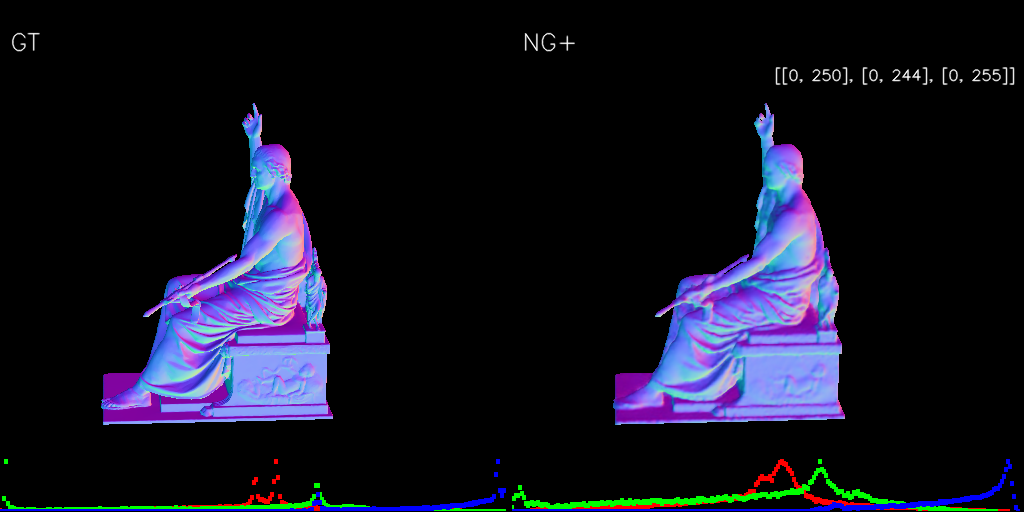
\includegraphics[width=\textwidth]{./pic/00349.gt.ngplus.png}}
%	\label{fig:washington_gt_ngpred}
%	\caption{Left: Ground truth normal map; Right: Predicted normal map based on model "NG"}
%\end{figure}

To further visualize the error of predicted normal map, figure \ref{fig:canny_edge_details} shows the angle error of normal map. 
It is obvious to see, that the error goes higher in the coarse surface, like fingers, gown and relief. Oppositely, the error goes lower in the smooth surface, like the arm, face, and foot. The coarse surface are mainly the boundaries, or edges, which can be extract efficiently using edge detection algorithms, like Canny Edge detector. Figure \ref{fig:canny_edge_details} shows the detected edge of ground truth using Canny Edge Detector.

%\begin{figure}[!h]
%	\centering
%	{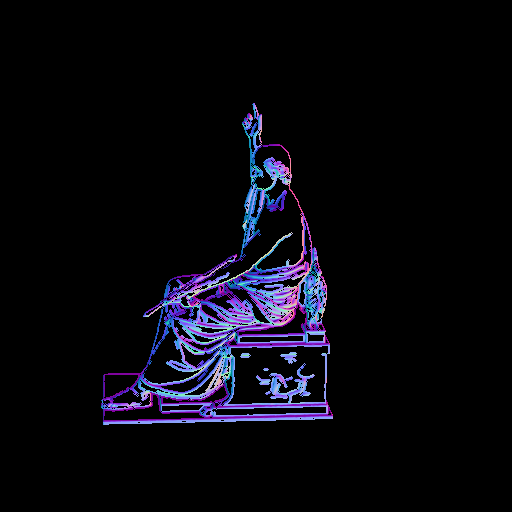
\includegraphics[width=0.45\textwidth]{./pic/00349.hpf0.png}}
%	{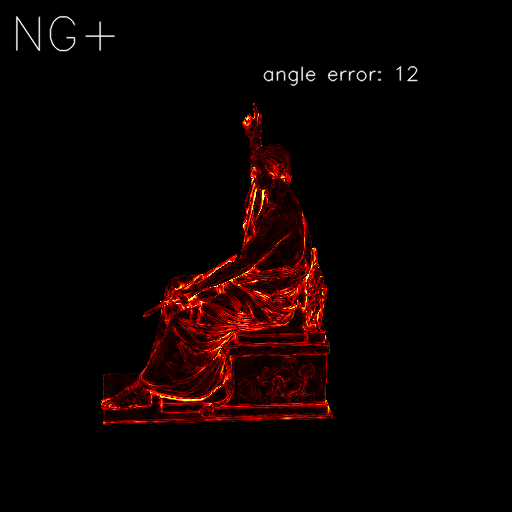
\includegraphics[width=0.45\textwidth]{./pic/00349.error.png}}
%	\label{fig:canny_edge_details}
%	\caption{Left: Normal Map; Middle: Detected Edge of Normal Map using Canny Edge Detection Algorithm; Right: Error of predicted normal map.}
%\end{figure}


\section{Detailed Gated ResNet Normal Neural Network}
Use edge detector algorithms for further improvement.